\section*{Описание экспериментальной установки}

Схема экспериментальной установки приведена на рисунке:

\begin{figure}[H]
	\centering
	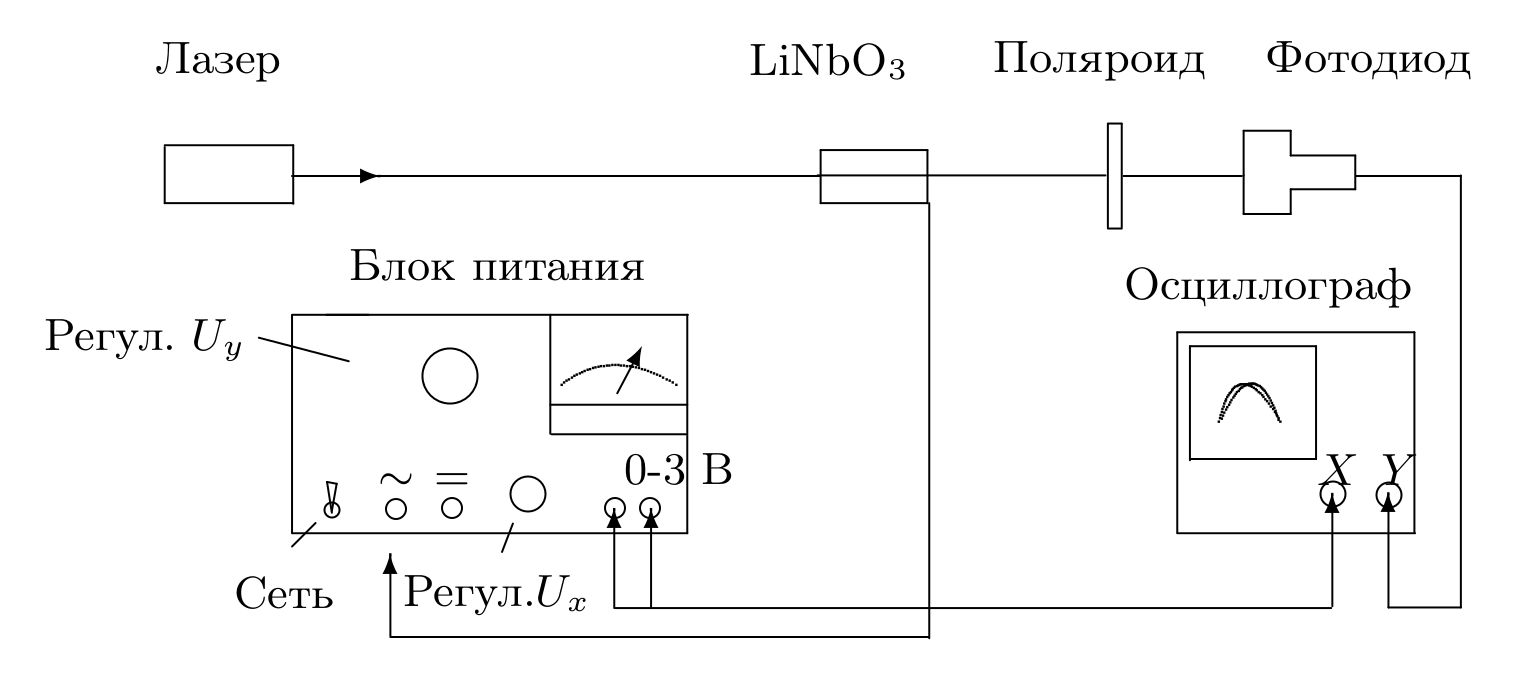
\includegraphics[width=0.8\textwidth]{../Изображения/facility.png}
	\caption{Схема экспериментальной установки}
\end{figure}

Луч света от лазера со встроенным вертикальным поляризатором попадает на кювету с кристаллом необата лития. Перед кюветой можно разместить матовую рассеивающую пластинку. Главная оптическая ось кристалла ориентирована вдоль направления распространения луча. После кюветы расположен поляроид. Результат интерференции наблюдается на экране. На кристалл можно подавать высоковольтное постоянное и переменное напряжение с помощью источника напряжения. Если подавать на кристалл переменное напряжение, то для исследования результата интерференции используется фотодиод, выход которого подключается к одному каналу осциллографа. Ко второму входу осциллографа подключается сигнал с источника напряжение.